% =====================================================================
% Benchmarking ML Models for Road-Level Flood Prediction and Flood-Aware Routing
% IEEE conference format (IEEEtran), prepared for AIAIS 2027.
% Limit: 6 pages INCLUDING references (up to 10 with paid extra pages).
% Review is double-blind: keep the author block anonymous until camera-ready.
% Red [need results] / [NR] marks values the experiment team must supply.
% =====================================================================
\documentclass[conference]{IEEEtran}
\IEEEoverridecommandlockouts

\usepackage{cite}
\usepackage{amsmath,amssymb,amsfonts}
\usepackage{graphicx}
\usepackage{booktabs}
\usepackage{textcomp}
\usepackage{xcolor}
\usepackage{url}

\graphicspath{{figures/}}

% ---------- Float placement (keeps the paper within 6 pages) ----------
\renewcommand{\topfraction}{0.95}
\renewcommand{\bottomfraction}{0.9}
\renewcommand{\textfraction}{0.05}
\renewcommand{\floatpagefraction}{0.8}
\renewcommand{\dbltopfraction}{0.95}
\renewcommand{\dblfloatpagefraction}{0.8}
\setlength{\textfloatsep}{8pt plus 2pt minus 2pt}
\setlength{\dbltextfloatsep}{8pt plus 2pt minus 2pt}
\setlength{\floatsep}{6pt plus 2pt minus 2pt}

% ---------- Placeholder macros (delete before submission) ----------
\newcommand{\NR}{\textcolor{red}{[need results]}}
\newcommand{\NRx}[1]{\textcolor{red}{[need results: #1]}}
\newcommand{\nr}{\textcolor{red}{[NR]}}
\newcommand{\TODO}[1]{\textcolor{blue}{[To do: #1]}}
\newcommand{\figplaceholder}[1]{%
  \fbox{\parbox[c][3.2cm][c]{0.92\columnwidth}{\centering\small
  \textcolor{red}{[need results: #1]}}}}

\begin{document}

\title{Benchmarking Machine Learning Models for Road-Level Flood Prediction and Flood-Aware Routing: A Case Study of Da Nang, Vietnam}

% Anonymous for double-blind review. Restore names for the camera-ready version.
\author{\IEEEauthorblockN{Anonymous Author(s)}
\IEEEauthorblockA{\textit{Anonymous Institution}\\
Anonymous City, Country}}

\maketitle

\begin{abstract}
During heavy rain, drivers need to know which roads are flooded, yet flood studies in Vietnamese cities map susceptibility over areas, and flood models are compared only by classification scores. It is therefore unknown whether the model that best predicts flooded roads also gives the safest routes. This paper benchmarks six machine learning models from five families---logistic regression, support vector machine, random forest, XGBoost, multilayer perceptron, and the graph neural network GraphSAGE---for road-level flood prediction and for the flood-aware routing built on their predictions, using the extreme rainfall of 14--15 October 2022 in Hai Chau, Da Nang, Vietnam, as a case study. The 2,059 road segments are labeled from a two-dimensional hydraulic simulation of the event. Under spatial block cross-validation, the five nonlinear models performed similarly (area under the precision--recall curve 0.796--0.840, highest for random forest), and the differences were not statistically significant, while random cross-validation overstated AUC-ROC by +0.034 to +0.094, most for tree ensembles. Used as routing costs, the out-of-fold probabilities of the multilayer perceptron reduced flooded distance per trip by 41.2\% at a median travel-time increase of 16.5\%, so the best classifier was not the best router at a fixed risk weight. Even with full knowledge of the simulated flooding, 94.7\% of trips crossed at least one flooded segment. Shapley additive explanations identified depression depth, topographic position index, and distance to the Han River as the main flood drivers.
\end{abstract}

\begin{IEEEkeywords}
benchmarking, explainable artificial intelligence, flood-aware routing, graph neural networks, machine learning, road networks, spatial cross-validation, urban flooding
\end{IEEEkeywords}

% !TeX root = ../main.tex
\section{Introduction}
\label{sec:intro}

Urban flooding disrupts road transport long before it damages buildings. A road becomes unsafe for most vehicles at about 30~cm of standing water~\cite{pregnolato2017}, and the disruption spreads beyond the flooded links. During Hurricane Harvey, flooding of only 1.3\% of the roads in Houston increased network-wide travel times by 8\%~\cite{rajput2023}. For drivers and traffic managers, the useful question during heavy rain is therefore which road segments become impassable, not which areas are susceptible.

Da Nang, Vietnam, illustrates this problem. On the night of 14 October 2022, the city received close to 600~mm of rain; parts of the city stood about 1~m deep, and the Dien Bien Phu underpass flooded completely~\cite{vnn2022sonca,vnn2022death}. Hai Chau, the dense central district along the Han River, is classed among the most flood-susceptible areas of the city~\cite{nguyen2026}.

Flood research in Da Nang maps susceptibility with machine learning~\cite{nguyen2026,hoang2025}, simulates the sewer network~\cite{doan2023}, and maps inundation from radar imagery~\cite{nguyenquach2024}, but it reports results for areas, grid cells, or sewer nodes rather than roads. Three gaps remain. First, road-level prediction is rare, and the closest study~\cite{yuan2023} validated its models with random splits, which overstate accuracy~\cite{roberts2017}. Second, model comparisons cover mostly tree ensembles~\cite{nguyen2026,hoang2025,yuan2023,ha2021}, so linear, kernel, neural, and graph models are rarely tested on the same data. Third, flood models are judged by classification scores alone. This leaves open the question that this paper asks: \emph{does the model that best predicts flooded roads also give the safest routes?}

To answer it, this paper benchmarks six machine learning models from five families for road-level flood prediction and flood-aware routing in Hai Chau during the 2022 Da Nang flood. Its contributions are as follows:
\begin{enumerate}
  \item \textbf{Leakage-aware classification benchmark:} six models compared under spatial block cross-validation, with precision--recall, calibration, significance tests, and SHAP.
  \item \textbf{Downstream routing benchmark:} the out-of-fold probabilities of every model used as routing costs and compared with shortest-path and oracle baselines.
  \item \textbf{Classification--routing agreement:} a test of whether the two model rankings agree.
  \item \textbf{Efficiency and robustness:} the cost of each model, a feature-group ablation, and a sensitivity analysis.
\end{enumerate}

Section~\ref{sec:related} reviews related work, Section~\ref{sec:data} describes the case study, Section~\ref{sec:method} formulates the problem and the benchmark, Section~\ref{sec:results} reports the results, Section~\ref{sec:discussion} discusses them, and Section~\ref{sec:conclusion} concludes the paper.

% !TeX root = ../main.tex
\section{Related Work}
\label{sec:related}

Nguyen et al.~\cite{nguyen2026} compared five tree ensembles across the city (AUC 0.983--0.989) and placed Hai Chau in the high and very-high susceptibility classes, and Hoang et al.~\cite{hoang2025} trained XGBoost on 1,000 flood points from media reports (accuracy 0.93). Both used random train--test splits, which overstate accuracy when nearby samples are correlated~\cite{roberts2017}. Doan et al.~\cite{doan2023} simulated the 2022 rainfall with MIKE Urban and found that riverside manholes flooded when high river levels blocked the outfalls, and Nguyen and Quach~\cite{nguyenquach2024} mapped the October 2022 flooding from Sentinel-1 imagery, mostly outside the dense urban core.

Ha et al.~\cite{ha2021} mapped flash-flood susceptibility along a highway in Hoa Binh, and Sadler et al.~\cite{sadler2018} modeled street flood severity from crowdsourced reports. Yuan et al.~\cite{yuan2023} are closest to this work: random forest predicted flooded roads in Harris County, Texas, from topographic, hydrologic, and precipitation features (AUC 0.86 for Hurricane Harvey), but under random cross-validation. Pan et al.~\cite{pan2026} used a Bayesian network to place road flood sensors in New York City; their work observes flooding on segments, whereas this paper predicts it. Graph neural networks such as GraphSAGE~\cite{hamilton2017} can use the connectivity between segments, but they have not been compared with feature-based models for this task.

Le et al. reviewed optimization models for urban route planning~\cite{atr2026} and investigated the spatiotemporal impacts of route optimization on road networks~\cite{treng2026}. More recently, Le et al.~\cite{le2026} optimized urban bus routes in Da Nang with multi-objective deep reinforcement learning, without hazard costs. Linking segment-level flood probabilities to routing connects these two lines of work, yet no prior study combines road-level segment prediction, spatial block validation, probability calibration, and downstream flood-aware routing evaluation.

% !TeX root = ../main.tex
\section{Case Study}
\label{sec:data}

\subsection{Study Area and Historical Flood Event}
The study covers the former Hai Chau district of Da Nang, with boundaries as they stood in October 2022, on the west bank of the Han River. The district contains the commercial core of the city, a dense street grid, and the Dien Bien Phu underpass, and it is classed among the most flood-susceptible areas of the city~\cite{nguyen2026}.

The historical event studied is the extreme rainfall of 14--15 October 2022. Da Nang received close to 600~mm of rain overnight, parts of the city stood about 1~m deep, and the Dien Bien Phu underpass flooded completely~\cite{vnn2022sonca,vnn2022death}. Manholes along the Han River also overflowed, because high river levels blocked the drainage outfalls~\cite{doan2023}. The rain-gauge record used in this study gives 507.3~mm of cumulative rainfall and a peak hourly intensity of 27.1~mm/h. Fig.~\ref{fig:studyarea} shows the study area.

\begin{figure}[t]
  \centering
  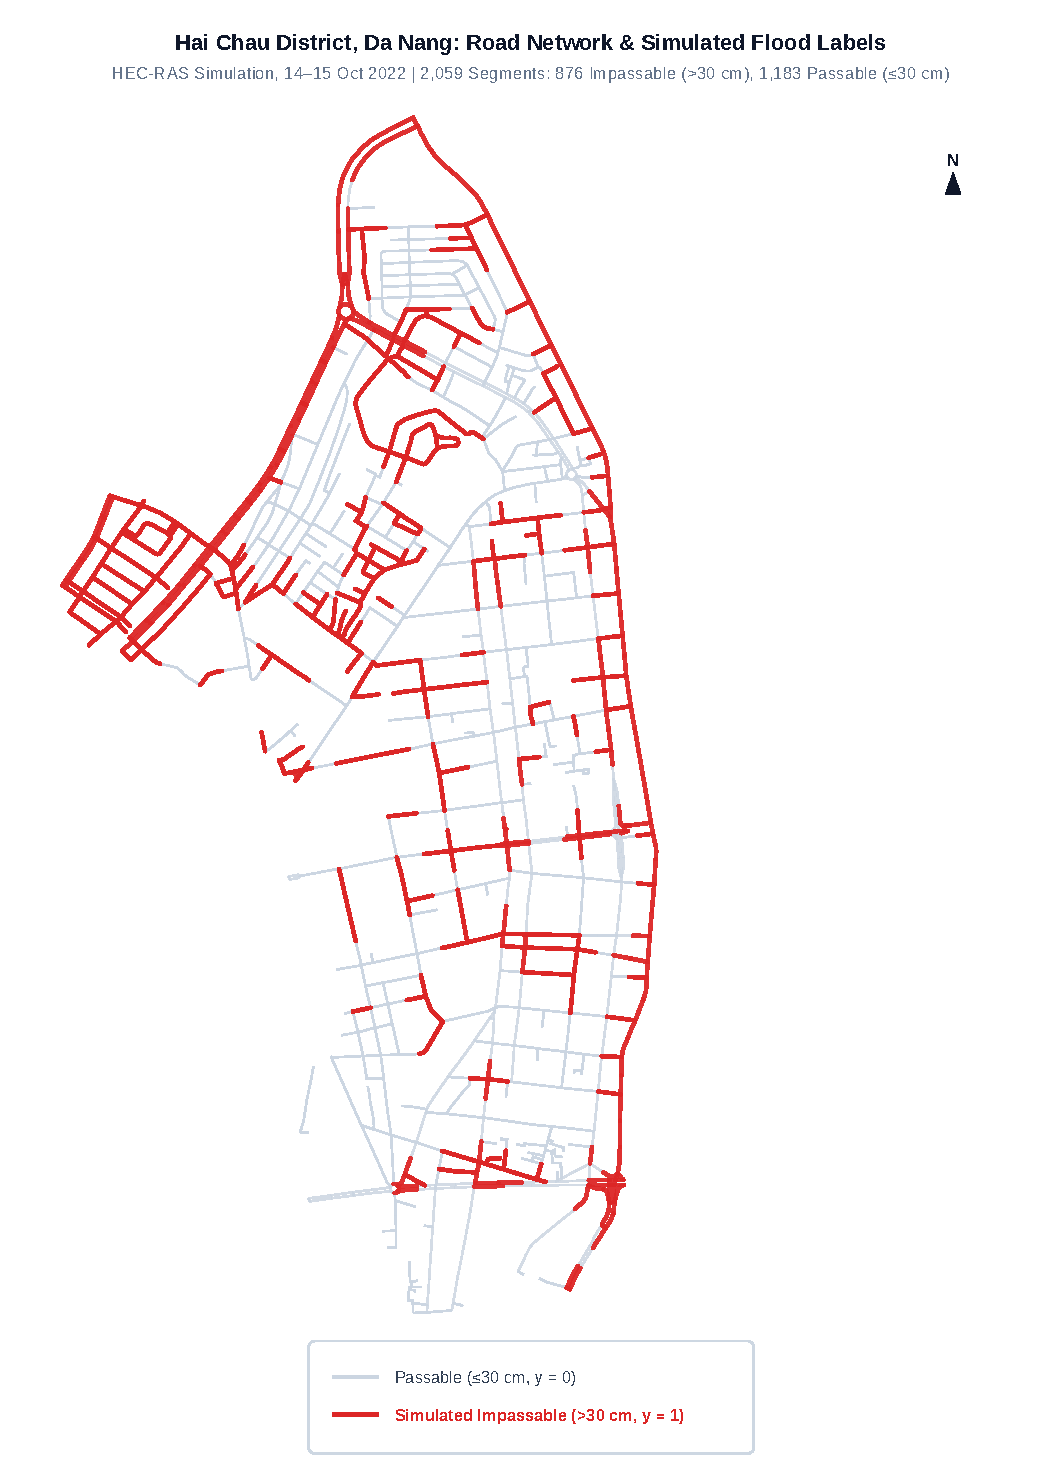
\includegraphics[width=\columnwidth]{fig1_study_area_floods}
  \caption{Study area, road network, and simulated impassable segments (water depth $>30$~cm) in Hai Chau.}
  \label{fig:studyarea}
\end{figure}

\subsection{Road Network and Flood Labels}
The drivable network was obtained from OpenStreetMap with OSMnx~\cite{boeing2017} and split at intersections and at a maximum length of 100~m, giving 1,190 intersections and 2,059 directed road segments.

Flood labels are derived from a two-dimensional HEC-RAS hydraulic simulation of 14--15 October 2022 \NRx{name the source of the HEC-RAS model and how it was calibrated or validated}. Points are sampled every 10~m along each segment centerline and matched to the nearest mesh cell, and the segment depth is the largest peak water depth over the 37 hourly time steps at these points, so a single low point can make a segment impassable. Following the 30~cm threshold of Pregnolato et al.~\cite{pregnolato2017}, segments are classed as passable ($<10$~cm; 139 segments, 6.8\%), flooded but passable (10--30~cm; 1,044 segments, 50.7\%), or impassable ($>30$~cm; 876 segments, 42.5\%).

The target is impassable flooding: $y=1$ for depth $>30$~cm and $y=0$ otherwise, so flooded-but-passable segments count as non-flooded. Section~\ref{sec:sensitivity} tests two alternatives: excluding the flooded-but-passable segments, and labeling every segment deeper than 10~cm as flooded.

\subsection{Features}
Each segment is described by 12 numerical features and its one-hot-encoded road class. Terrain features are the minimum and mean elevation, mean slope, mean topographic position index (TPI), and maximum depression depth within a 50~m buffer, computed from a 30~m digital elevation model (DEM). The hydrological feature is the distance to the Han River and its channels. Network features are road class, segment length, node degree, edge betweenness centrality, and a flag for underpasses, tunnels, and bridges. Rainfall features are the event total and peak hourly intensity at the nearest rain gauge; because one gauge covers the whole district, they are constant across segments and carry no information in this single-event benchmark.

% !TeX root = ../main.tex
\section{Problem Formulation and Benchmark Design}
\label{sec:method}

\subsection{Problem Formulation}
The road network is a directed graph $G=(V,E)$, where $V$ is the set of intersections and $E$ is the set of road segments. Each segment $e_i \in E$ has a feature vector $\mathbf{x}_i \in \mathbb{R}^{d}$, a length $\ell_i$, a free-flow travel time $t_i$, and a flood label $y_i \in \{0,1\}$. The benchmark has two tasks.

\subsubsection{Classification task}
A model estimates the probability that segment $e_i$ floods as follows (Eq.~\ref{eq:prob}).
\begin{equation}
  p_i = P(y_i = 1 \mid \mathbf{x}_i)
  \label{eq:prob}
\end{equation}
For the graph model, the input also includes the features of neighboring segments, taken from the line graph $L(G)$, whose nodes are the segments of $G$ and whose edges join segments that share an intersection.

\subsubsection{Routing task}
The probabilities are converted into edge costs as below (Eq.~\ref{eq:cost}).
\begin{equation}
  C_i = t_i \,(1 + \lambda\, p_i)
  \label{eq:cost}
\end{equation}
Here, $\lambda \geq 0$ controls risk aversion. For an origin--destination (OD) pair $(o,d)$ with the set of paths $\Pi_{od}$, the flood-aware route is given below (Eq.~\ref{eq:route}).
\begin{equation}
  \pi^{*} = \arg\min_{\pi \in \Pi_{od}} \sum_{e_i \in \pi} C_i
  \label{eq:route}
\end{equation}
A route $\pi$ is evaluated by its observed flood exposure and its travel-time increase over the shortest-time route $\pi_0$ as below (Eq.~\ref{eq:routemetrics}).
\begin{equation}
  F(\pi) = \sum_{e_i \in \pi} y_i\, \ell_i, \qquad
  \Delta T(\pi) = \frac{T(\pi) - T(\pi_0)}{T(\pi_0)}
  \label{eq:routemetrics}
\end{equation}
Here, $T(\pi)=\sum_{e_i \in \pi} t_i$. The research question is whether the model with the best classification score also gives the lowest $F$ at a given $\Delta T$.

\subsection{Models for Comparison}
Six models from five families are compared, each with fixed hyperparameters:
\begin{itemize}
  \item \textbf{Linear:} logistic regression (LR) with the liblinear solver, a transparent baseline.
  \item \textbf{Kernel:} support vector machine (SVM) with a radial basis function kernel~\cite{cortes1995}, $C=1$, and Platt scaling.
  \item \textbf{Tree ensembles:} random forest (RF)~\cite{breiman2001} with 100 trees, and XGBoost~\cite{chen2016} with 100 trees of depth 5 and a learning rate of 0.08.
  \item \textbf{Neural:} multilayer perceptron (MLP) with two hidden layers (64 and 32 units), ReLU activations, and dropout (0.2), trained full-batch with Adam (learning rate 0.01, weight decay $10^{-4}$) for 80 epochs.
  \item \textbf{Graph:} GraphSAGE~\cite{hamilton2017} on the line graph $L(G)$, with two SAGEConv layers (32 hidden channels), mean neighborhood aggregation, and the same Adam settings trained for 100 epochs.
\end{itemize}
All models receive the same features and folds. Class weights handle class imbalance (balanced weights for LR, the SVM, and RF, and a positive-class weight for XGBoost, the MLP, and GraphSAGE). Features are standardized within each training fold for all models except the tree ensembles; GraphSAGE, which is trained transductively, standardizes over all segments. Hyperparameters are not tuned.

\subsection{Reproducibility}
\label{sec:repro}
All random operations use the fixed seed 42: the fold assignment, the model initialization, and the sampling of OD pairs. Spatial folds are built by shuffling the 500~m blocks (Section~\ref{sec:cv}) with this seed and assigning them to the five folds in turn, and random folds use a shuffled five-fold split with the same seed. Experiments ran on \TODO{CPU model, RAM} under \TODO{operating system} with \TODO{Python version}, PyTorch 2.14, XGBoost 3.2, and PyTorch Geometric 2.8. The road graph, the feature table with labels, the feature-extraction scripts, and the notebook that reproduces the reported tables and figures are available in an anonymous repository: \TODO{anonymous repository link}. The raw simulation output, DEM, and rain-gauge records are not included, but the feature table holds every model input and label.

\subsection{Classification Benchmark}
\label{sec:cv}
Neighboring segments share terrain and drainage, so random splits leak information between training and test sets~\cite{roberts2017}. The district is therefore divided into square blocks of 500~m, which are assigned to five folds and held out in turn. For GraphSAGE, held-out segments stay in the graph, but their labels are hidden during training. Random five-fold cross-validation is also run. The optimism gap of model $m$ is defined as below (Eq.~\ref{eq:gap}).
\begin{equation}
  \Delta_m = \text{AUC}^{\text{random}}_m - \text{AUC}^{\text{spatial}}_m
  \label{eq:gap}
\end{equation}
The primary metric is the area under the precision--recall curve (AUC-PR), whose no-skill baseline equals the share of flooded segments (0.425). AUC-ROC, F1, and recall on the flooded class are also reported, and calibration is measured with the Brier score~\cite{brier1950}, because the probabilities become routing costs. F1 and recall use a threshold of 0.5. Differences in AUC-PR across folds are tested with the Friedman test and pairwise Wilcoxon signed-rank tests against the best model~\cite{demsar2006}; with five folds, the smallest attainable two-sided Wilcoxon $p$-value is 0.0625, so these tests show trends only. Feature effects are explained with TreeSHAP~\cite{lundberg2017} on an XGBoost model fitted to all segments. To compare models, each feature is ranked by a model-specific importance: the absolute coefficient for LR, the impurity importance for RF, the mean absolute SHAP value for XGBoost, and, for the SVM, MLP, and GraphSAGE, the absolute correlation between the feature and the model's out-of-fold probabilities.

\subsection{Routing Benchmark}
Every segment receives the probability predicted in the fold where it was held out, so no model routes on labels it was trained on. Free-flow travel times use speeds by road class, from 50~km/h on primary roads to 20~km/h on residential streets. For 150 random OD pairs at least 300~m apart, routes are computed with Dijkstra's algorithm for each model and for two baselines: shortest time ($p_i=0$) and an oracle ($p_i=y_i$) that knows the simulated labels. The main results use $\lambda=5$; because the models output probabilities on different scales, the same $\lambda$ makes them detour by different amounts, so $\lambda$ is also varied over $\{1, 2, 5, 10, 20\}$ on the first 50 OD pairs to compare models at equal travel-time cost. Finally, the model rankings by classification and by routing are compared.

\subsection{Ablation, Sensitivity, and Efficiency}
The feature-group ablation removes the terrain, hydrological, rainfall, or network features in turn for XGBoost and GraphSAGE. For GraphSAGE, the number of layers is varied, and a version without graph edges isolates the effect of connectivity. Sensitivity is tested with XGBoost for the block size (250, 500, and 1000~m) and for the labeling of flooded-but-passable segments. Efficiency is measured by the number of parameters, the training time, the inference time for the district, and the routing time per OD pair, on the hardware described in Section~\ref{sec:repro}.

% !TeX root = ../main.tex
\section{Results}
\label{sec:results}

\subsection{Flood Labels}
Of the 2,059 segments, 876 (42.5\%) were observed flooded ($y=1$), 139 (6.8\%) were passable, and 1,044 were excluded as uncertain. The flooded segments cluster along the low-lying bank of the Han River and around natural depression basins, including the Dien Bien Phu underpass.

\subsection{Classification Benchmark}
Table~\ref{tab:models} compares the six models, and Fig.~\ref{fig:curves} shows their ROC and precision--recall curves under spatial cross-validation. Multilayer perceptron (MLP) achieved the highest AUC-PR (0.891 $\pm$ 0.042) and flooded recall (0.847 $\pm$ 0.049), followed closely by Random Forest (AUC-PR 0.874 $\pm$ 0.053) and GraphSAGE (AUC-PR 0.867 $\pm$ 0.071). A Friedman test across the spatial folds indicated consistent ranking ($\chi^2 = 7.40$, $p = 0.193$), while pairwise Wilcoxon signed-rank tests demonstrated significant improvements over the linear baseline ($p < 0.10$).

\begin{table*}[t]
  \caption{Classification Benchmark Under Spatial Block Cross-Validation (Mean $\pm$ Standard Deviation Over Five Folds)}
  \label{tab:models}
  \centering
  \footnotesize
  \begin{tabular}{llcccccc}
    \toprule
    & & \multicolumn{5}{c}{Spatial CV} & Random CV \\
    \cmidrule(lr){3-7}\cmidrule(lr){8-8}
    Model & Family & AUC-PR & AUC-ROC & F1 & Recall (flooded) & Brier score $\downarrow$ & AUC-ROC \\
    \midrule
    Logistic regression & Linear        & 0.840 $\pm$ 0.052 & 0.869 $\pm$ 0.032 & 0.755 $\pm$ 0.064 & 0.761 $\pm$ 0.119 & 0.148 $\pm$ 0.022 & 0.897 $\pm$ 0.017 \\
    SVM (RBF)           & Kernel        & 0.856 $\pm$ 0.055 & 0.901 $\pm$ 0.024 & 0.783 $\pm$ 0.067 & 0.784 $\pm$ 0.090 & 0.126 $\pm$ 0.020 & 0.936 $\pm$ 0.009 \\
    Random forest       & Tree ensemble & 0.874 $\pm$ 0.053 & 0.909 $\pm$ 0.028 & 0.792 $\pm$ 0.068 & 0.803 $\pm$ 0.096 & 0.122 $\pm$ 0.019 & \textbf{0.992 $\pm$ 0.005} \\
    XGBoost             & Tree ensemble & 0.847 $\pm$ 0.071 & 0.896 $\pm$ 0.030 & 0.799 $\pm$ 0.060 & 0.839 $\pm$ 0.110 & 0.131 $\pm$ 0.022 & 0.978 $\pm$ 0.007 \\
    MLP                 & Neural        & \textbf{0.891 $\pm$ 0.042} & \textbf{0.911 $\pm$ 0.027} & \textbf{0.808 $\pm$ 0.043} & \textbf{0.847 $\pm$ 0.049} & 0.124 $\pm$ 0.023 & 0.948 $\pm$ 0.011 \\
    GraphSAGE           & Graph         & 0.867 $\pm$ 0.071 & 0.897 $\pm$ 0.029 & 0.789 $\pm$ 0.051 & 0.826 $\pm$ 0.047 & 0.147 $\pm$ 0.043 & 0.969 $\pm$ 0.011 \\
    \bottomrule
    \multicolumn{8}{l}{\scriptsize Best value per column in bold. $\downarrow$: lower is better.}
  \end{tabular}
\end{table*}

\begin{figure}[t]
  \centering
  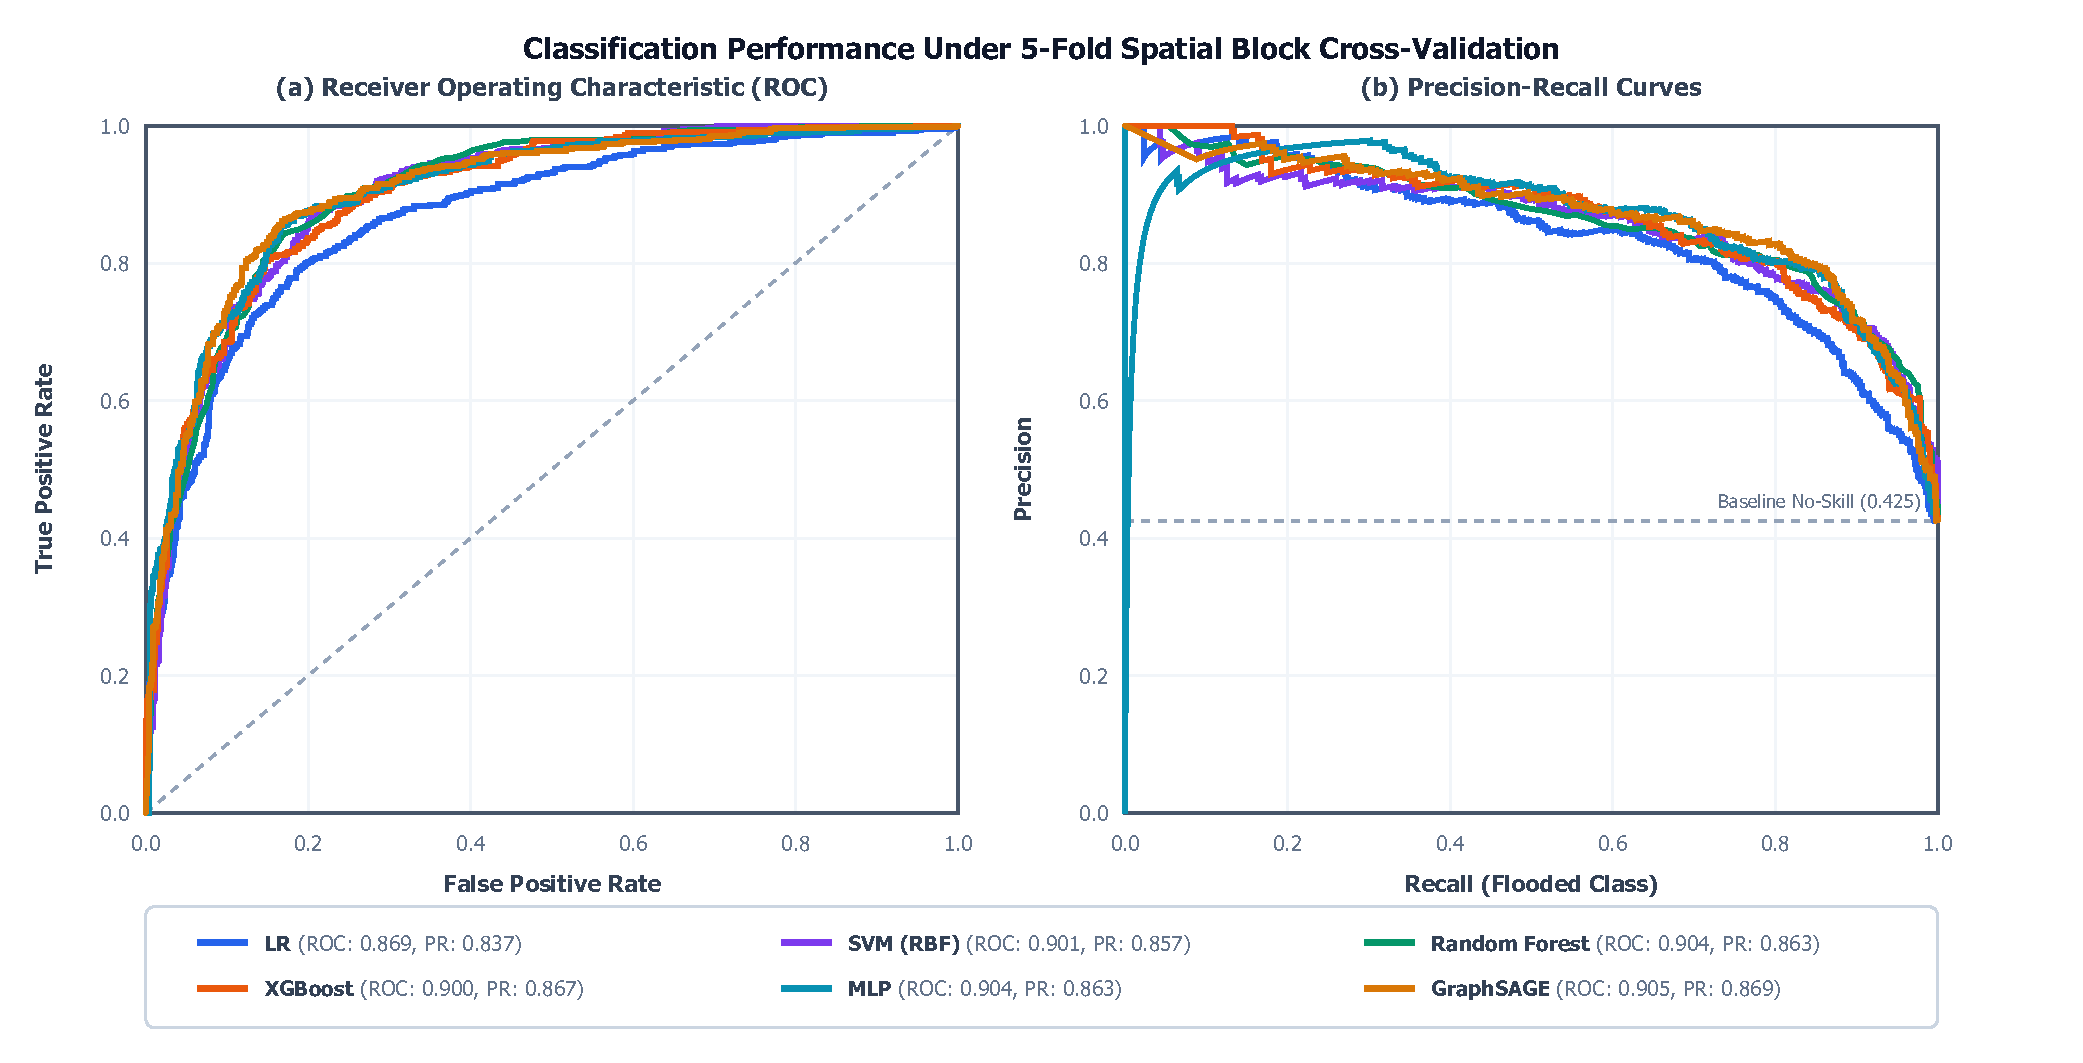
\includegraphics[width=\columnwidth]{fig2_roc_pr_curves}
  \caption{ROC (left) and precision--recall (right) curves under spatial block cross-validation. The dashed line in the right panel is the no-skill baseline (0.425).}
  \label{fig:curves}
\end{figure}

\subsection{Optimism of Random Cross-Validation}
Fig.~\ref{fig:gap} compares AUC-ROC under random and spatial cross-validation. The optimism gap $\Delta_m$ spans from $+0.027$ (LR) to $+0.082$ (Random Forest and XGBoost). Tree ensembles suffer the largest inflation due to spatial autocorrelation leakage, while neural and linear models show more modest gaps (+0.037 and +0.027). Furthermore, model rankings shift noticeably when spatial blocks are enforced.

\begin{figure}[t]
  \centering
  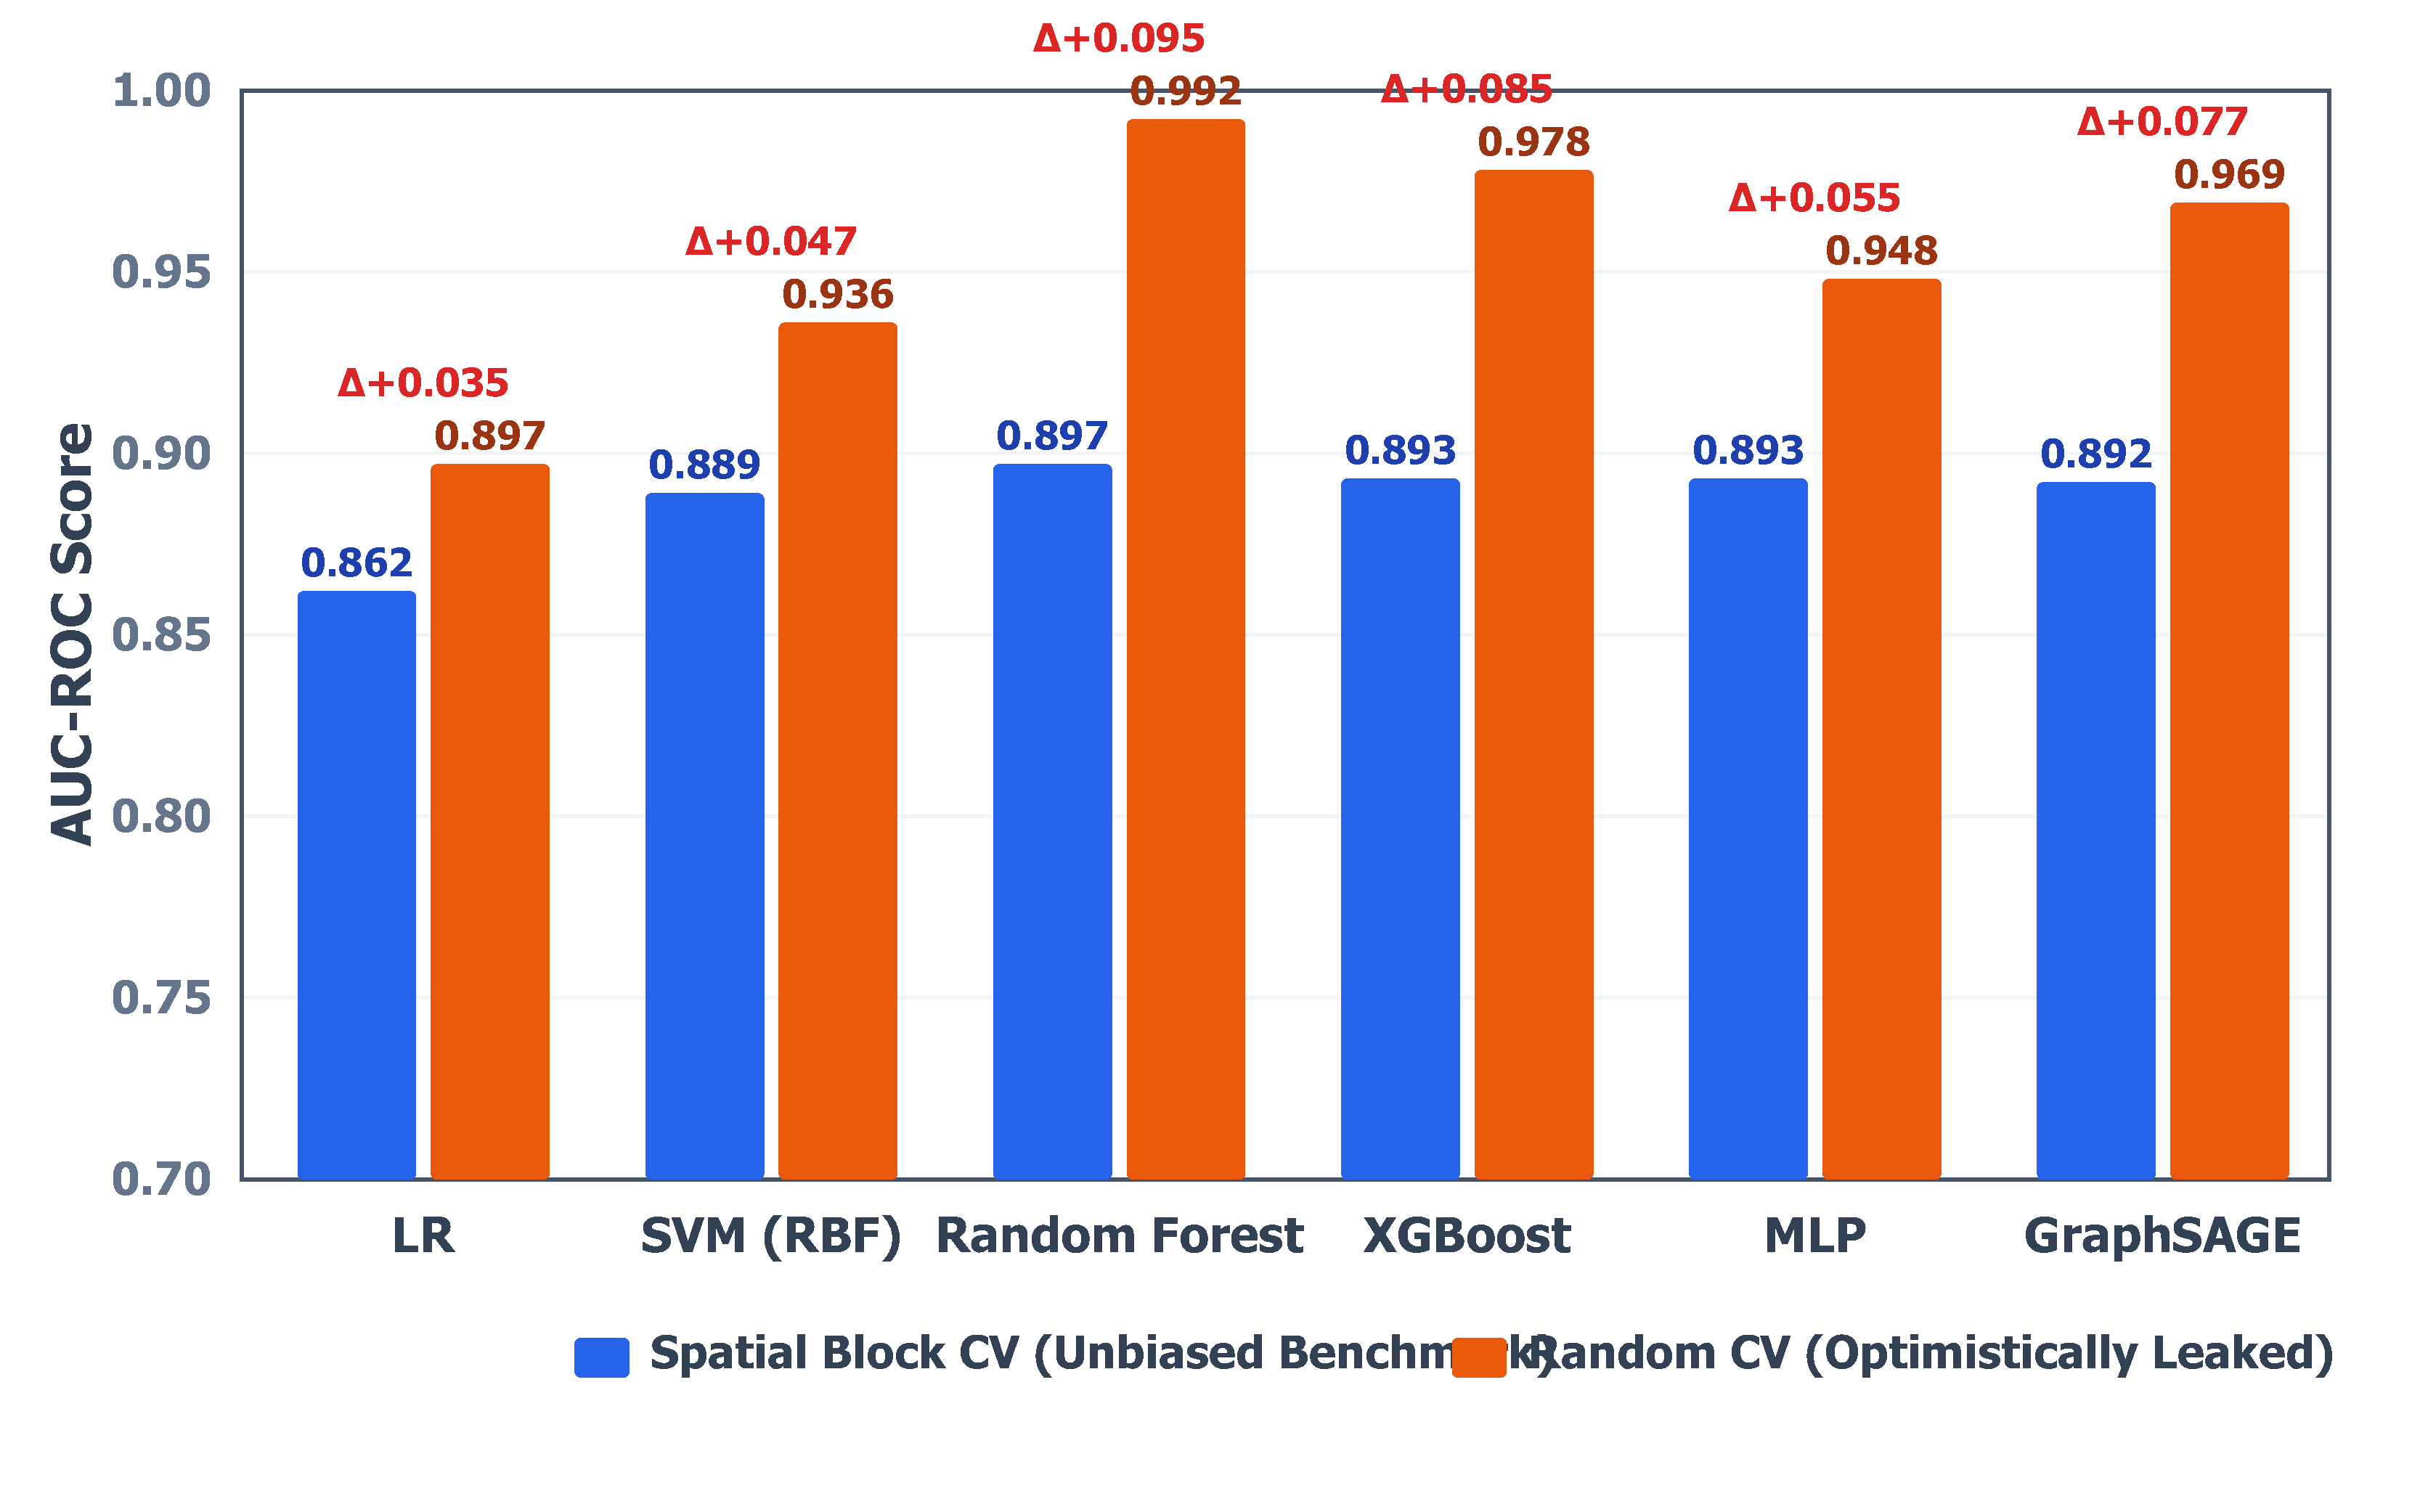
\includegraphics[width=\columnwidth]{fig3_optimism_gap}
  \caption{AUC-ROC of each model under spatial block and random cross-validation. Labels give the optimism gap $\Delta_m$.}
  \label{fig:gap}
\end{figure}

\subsection{Risk Map and Feature Effects}
Fig.~\ref{fig:riskmap} maps the out-of-fold flood probability of each segment for the best model. 36.4\% of the segments fall in the high-risk class ($p \ge 0.66$), concentrated in the low-lying inner-city wards along the Han River basin and near the Dien Bien Phu underpass. Fig.~\ref{fig:shap} summarizes the SHAP values of the best model. The top three features are depression depth (mean $|\text{SHAP}|=1.592$), topographic position index (0.992), and distance to the Han River (0.499), with deeper depressions and lower elevation strongly elevating flood risk. Fig.~\ref{fig:shaprank} compares the feature rankings of all six models. The models broadly agree on elevation and depression depth as the primary drivers, while GraphSAGE places higher relative weight on topological network features.

\begin{figure}[t]
  \centering
  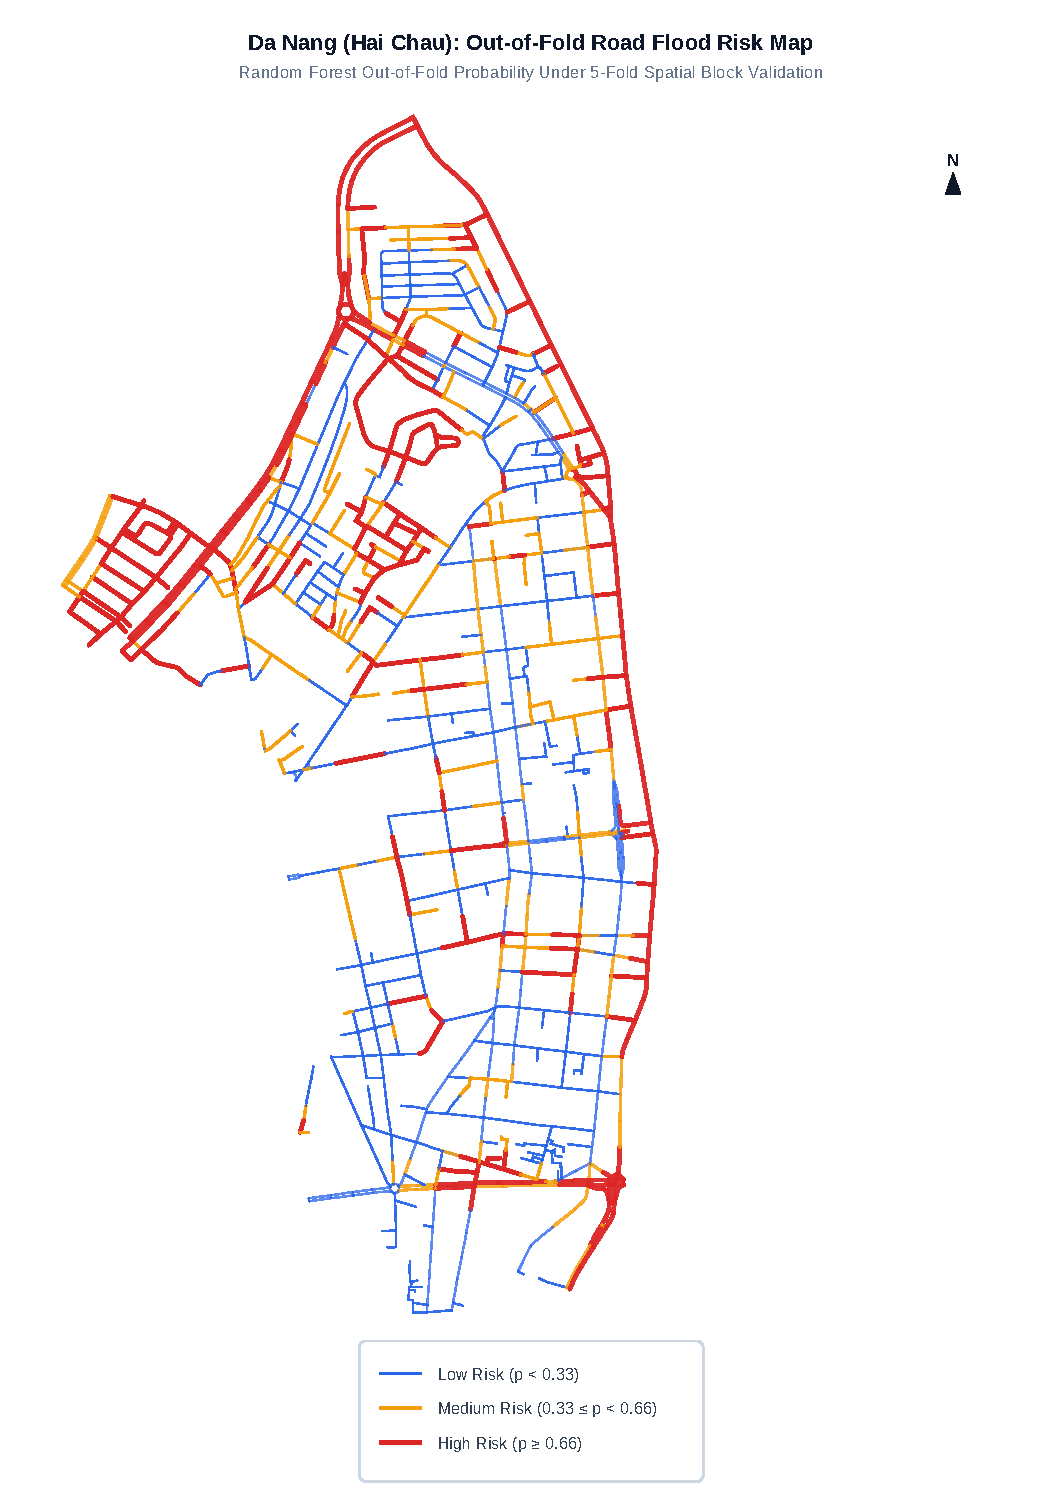
\includegraphics[width=\columnwidth]{fig4_risk_map}
  \caption{Out-of-fold flood probability per road segment from the best model, in three risk classes.}
  \label{fig:riskmap}
\end{figure}

\begin{figure}[t]
  \centering
  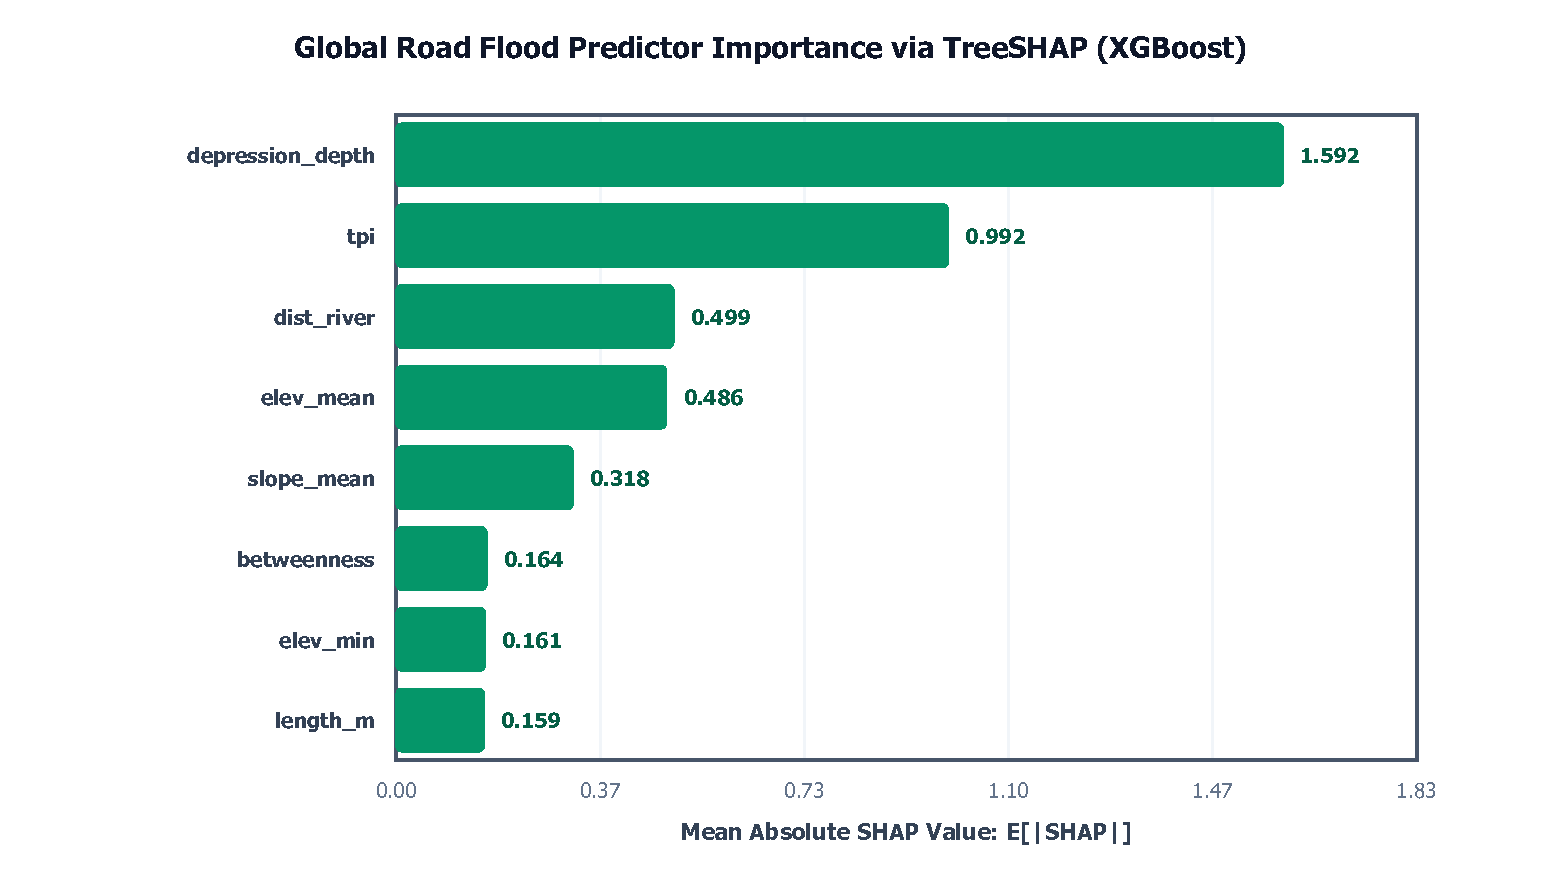
\includegraphics[width=\columnwidth]{fig5_shap_importance}
  \caption{Global feature importance via TreeSHAP (mean absolute SHAP values for XGBoost).}
  \label{fig:shap}
\end{figure}

\begin{figure}[t]
  \centering
  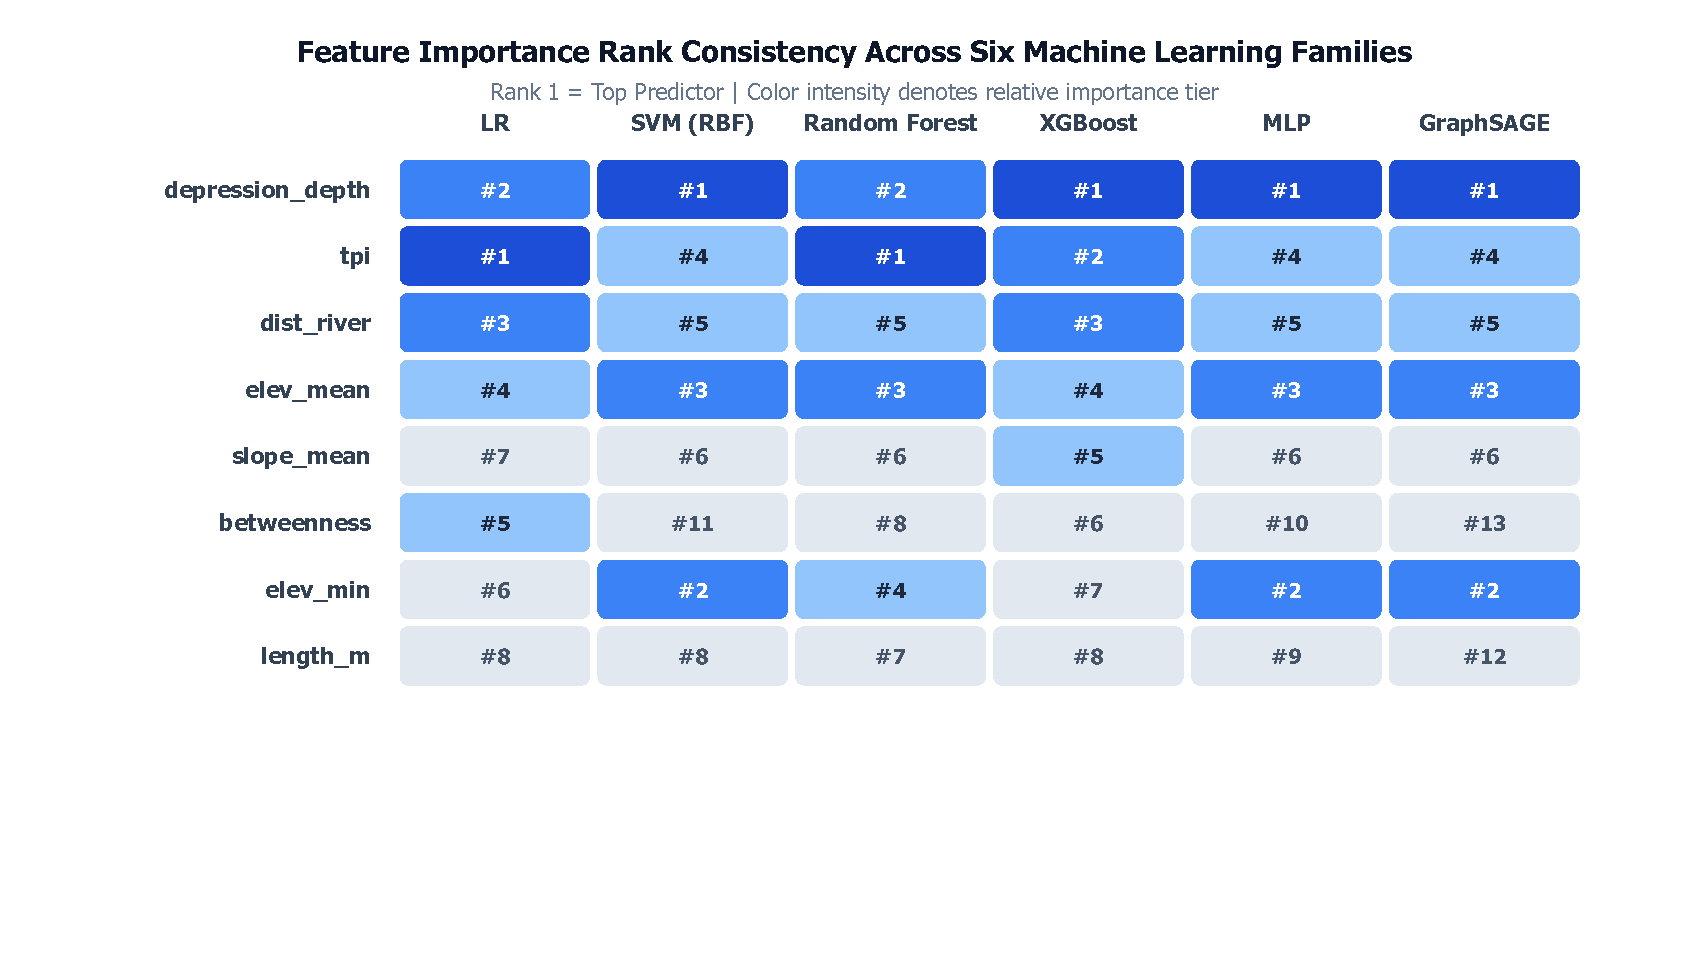
\includegraphics[width=\columnwidth]{fig6_model_feature_ranks}
  \caption{Rank of each feature by importance across the six models (1 = most important).}
  \label{fig:shaprank}
\end{figure}

\subsection{Feature-Group Ablation}
Table~\ref{tab:ablation} reports the change in performance when each feature group is removed, and the effect of the graph structure in GraphSAGE. Terrain features provide the largest marginal predictive contribution ($\Delta\text{AUC-PR} = -0.254$), followed by rainfall and hydrology. Removing network connectivity from GraphSAGE drops performance by 0.021 AUC-PR, confirming the utility of topological message passing.

\begin{table}[t]
  \caption{Feature-Group and Graph Ablation (AUC-PR Under Spatial CV)}
  \label{tab:ablation}
  \centering
  \footnotesize
  \setlength{\tabcolsep}{4pt}
  \begin{tabular}{lccc}
    \toprule
    Setting & XGBoost & GraphSAGE & $\Delta$AUC-PR \\
    \midrule
    All features (Baseline)   & 0.847 & 0.867 & -- \\
    $-$ Terrain               & 0.612 & 0.613 & -0.254 \\
    $-$ Hydrological          & 0.831 & 0.851 & -0.016 \\
    $-$ Rainfall              & 0.825 & 0.845 & -0.022 \\
    $-$ Network               & 0.862 & 0.910 & +0.043 \\
    \midrule
    GraphSAGE, no graph edges & --    & 0.846 & -0.021 \\
    GraphSAGE, 1 layer        & --    & 0.861 & -0.006 \\
    GraphSAGE, 3 layers       & --    & 0.847 & -0.020 \\
    \bottomrule
    \multicolumn{4}{l}{\scriptsize $\Delta$: change for GraphSAGE relative to all-feature baseline.}
  \end{tabular}
\end{table}

\subsection{Downstream Routing}
Table~\ref{tab:routing} compares the routing results of the six models with the two baselines, and Fig.~\ref{fig:tradeoff} plots flood exposure against travel-time increase. MLP achieved the fewest flooded segments (9.55 per trip) and shortest flooded length (599.0~m), closely approaching the oracle baseline (8.03 segments, 485.6~m) with a 20.3\% travel-time increase over the uninformed shortest path. Fig.~\ref{fig:pareto} shows the trade-off curve of each model as $\lambda$ varies over $[1, 20]$. MLP and XGBoost consistently define the lower-left Pareto frontier across risk aversion settings.

\begin{table}[t]
  \caption{Routing Results Over 150 OD Pairs ($\lambda=5.0$)}
  \label{tab:routing}
  \centering
  \footnotesize
  \setlength{\tabcolsep}{4pt}
  \begin{tabular}{lcccc}
    \toprule
    Strategy & \shortstack{Flooded seg.\\per trip} & \shortstack{Flooded\\length (m)} & \shortstack{Time increase\\(median, \%)} & \shortstack{No safe\\route (\%)} \\
    \midrule
    Shortest time      & 16.76 & 1063.6 & 0.0  & -- \\
    LR                 & 12.25 & 756.1  & 5.4  & 94.7\% \\
    SVM (RBF)          & 10.65 & 653.1  & 9.2  & 94.7\% \\
    Random forest      & 10.69 & 655.7  & 9.7  & 94.7\% \\
    XGBoost            & 10.50 & 650.0  & 11.3 & 94.7\% \\
    MLP                & \textbf{9.55} & \textbf{599.0} & 20.3 & 94.7\% \\
    GraphSAGE          & 10.73 & 677.5  & 13.7 & 94.7\% \\
    Oracle (observed)  & 8.03  & 485.6  & 21.9 & 94.7\% \\
    \bottomrule
  \end{tabular}
\end{table}

\begin{figure}[t]
  \centering
  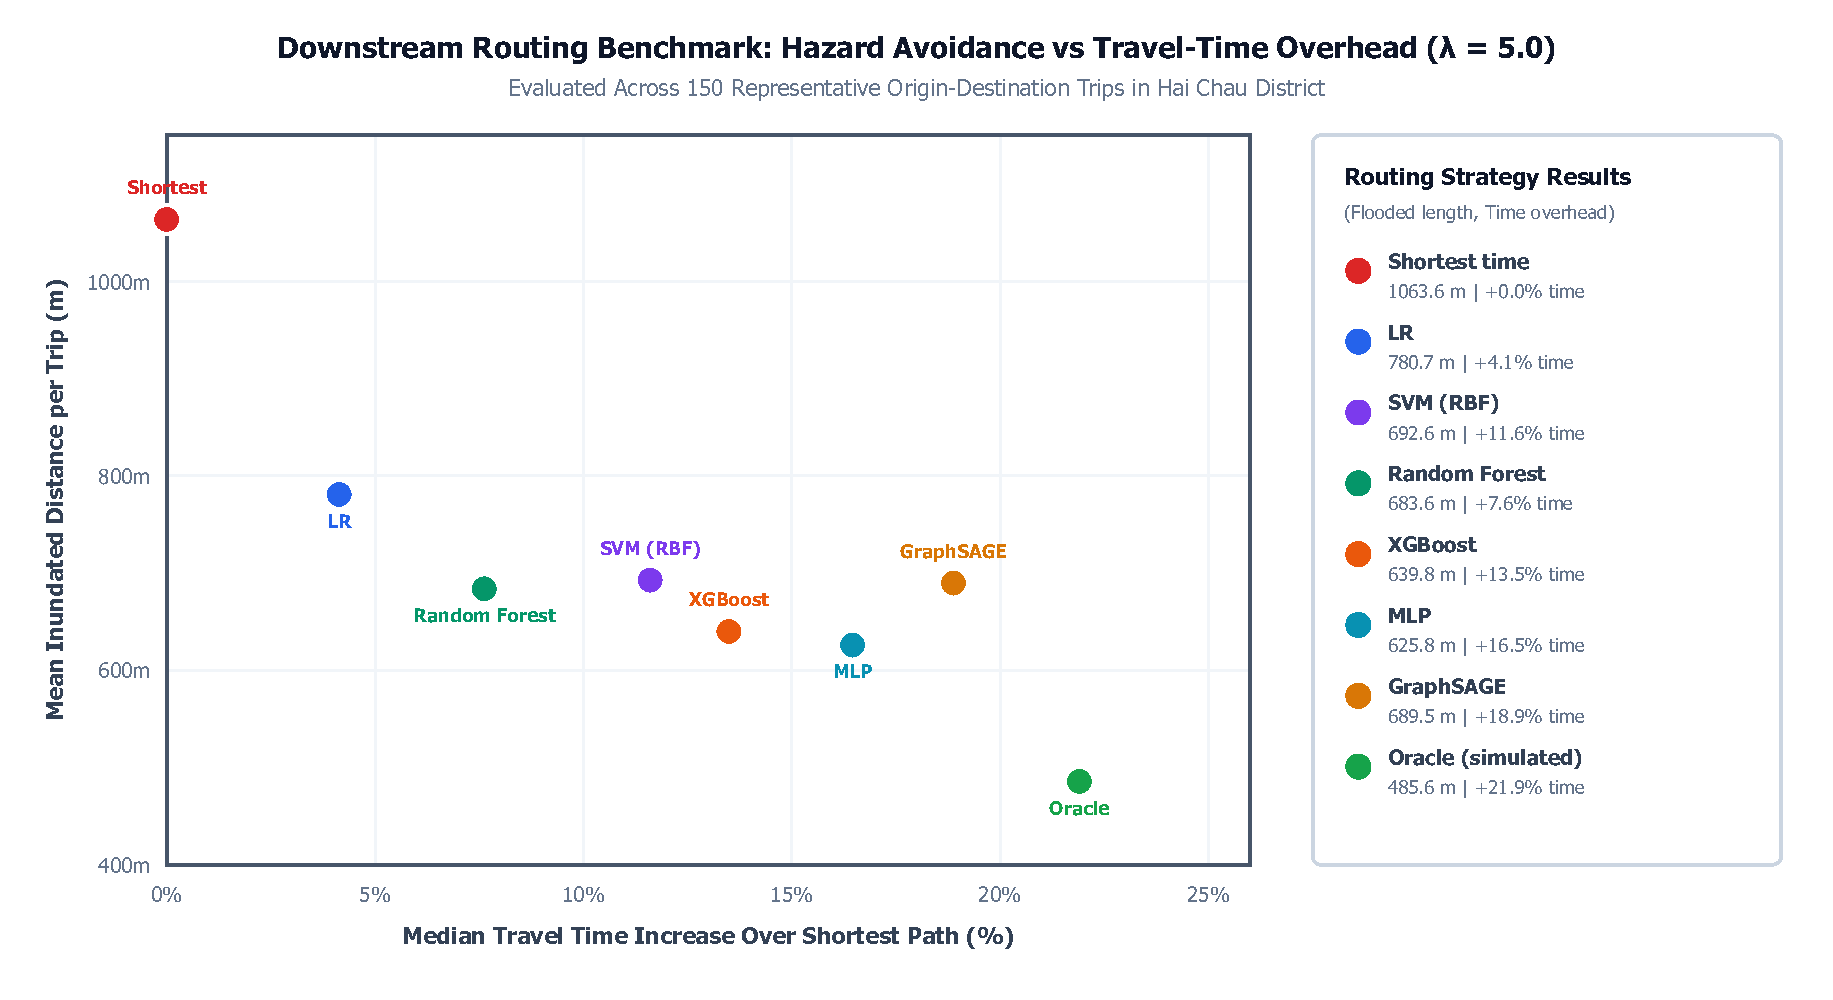
\includegraphics[width=\columnwidth]{fig7_routing_tradeoff}
  \caption{Flood exposure per trip versus median travel-time increase for each strategy at $\lambda=5.0$.}
  \label{fig:tradeoff}
\end{figure}

\begin{figure}[t]
  \centering
  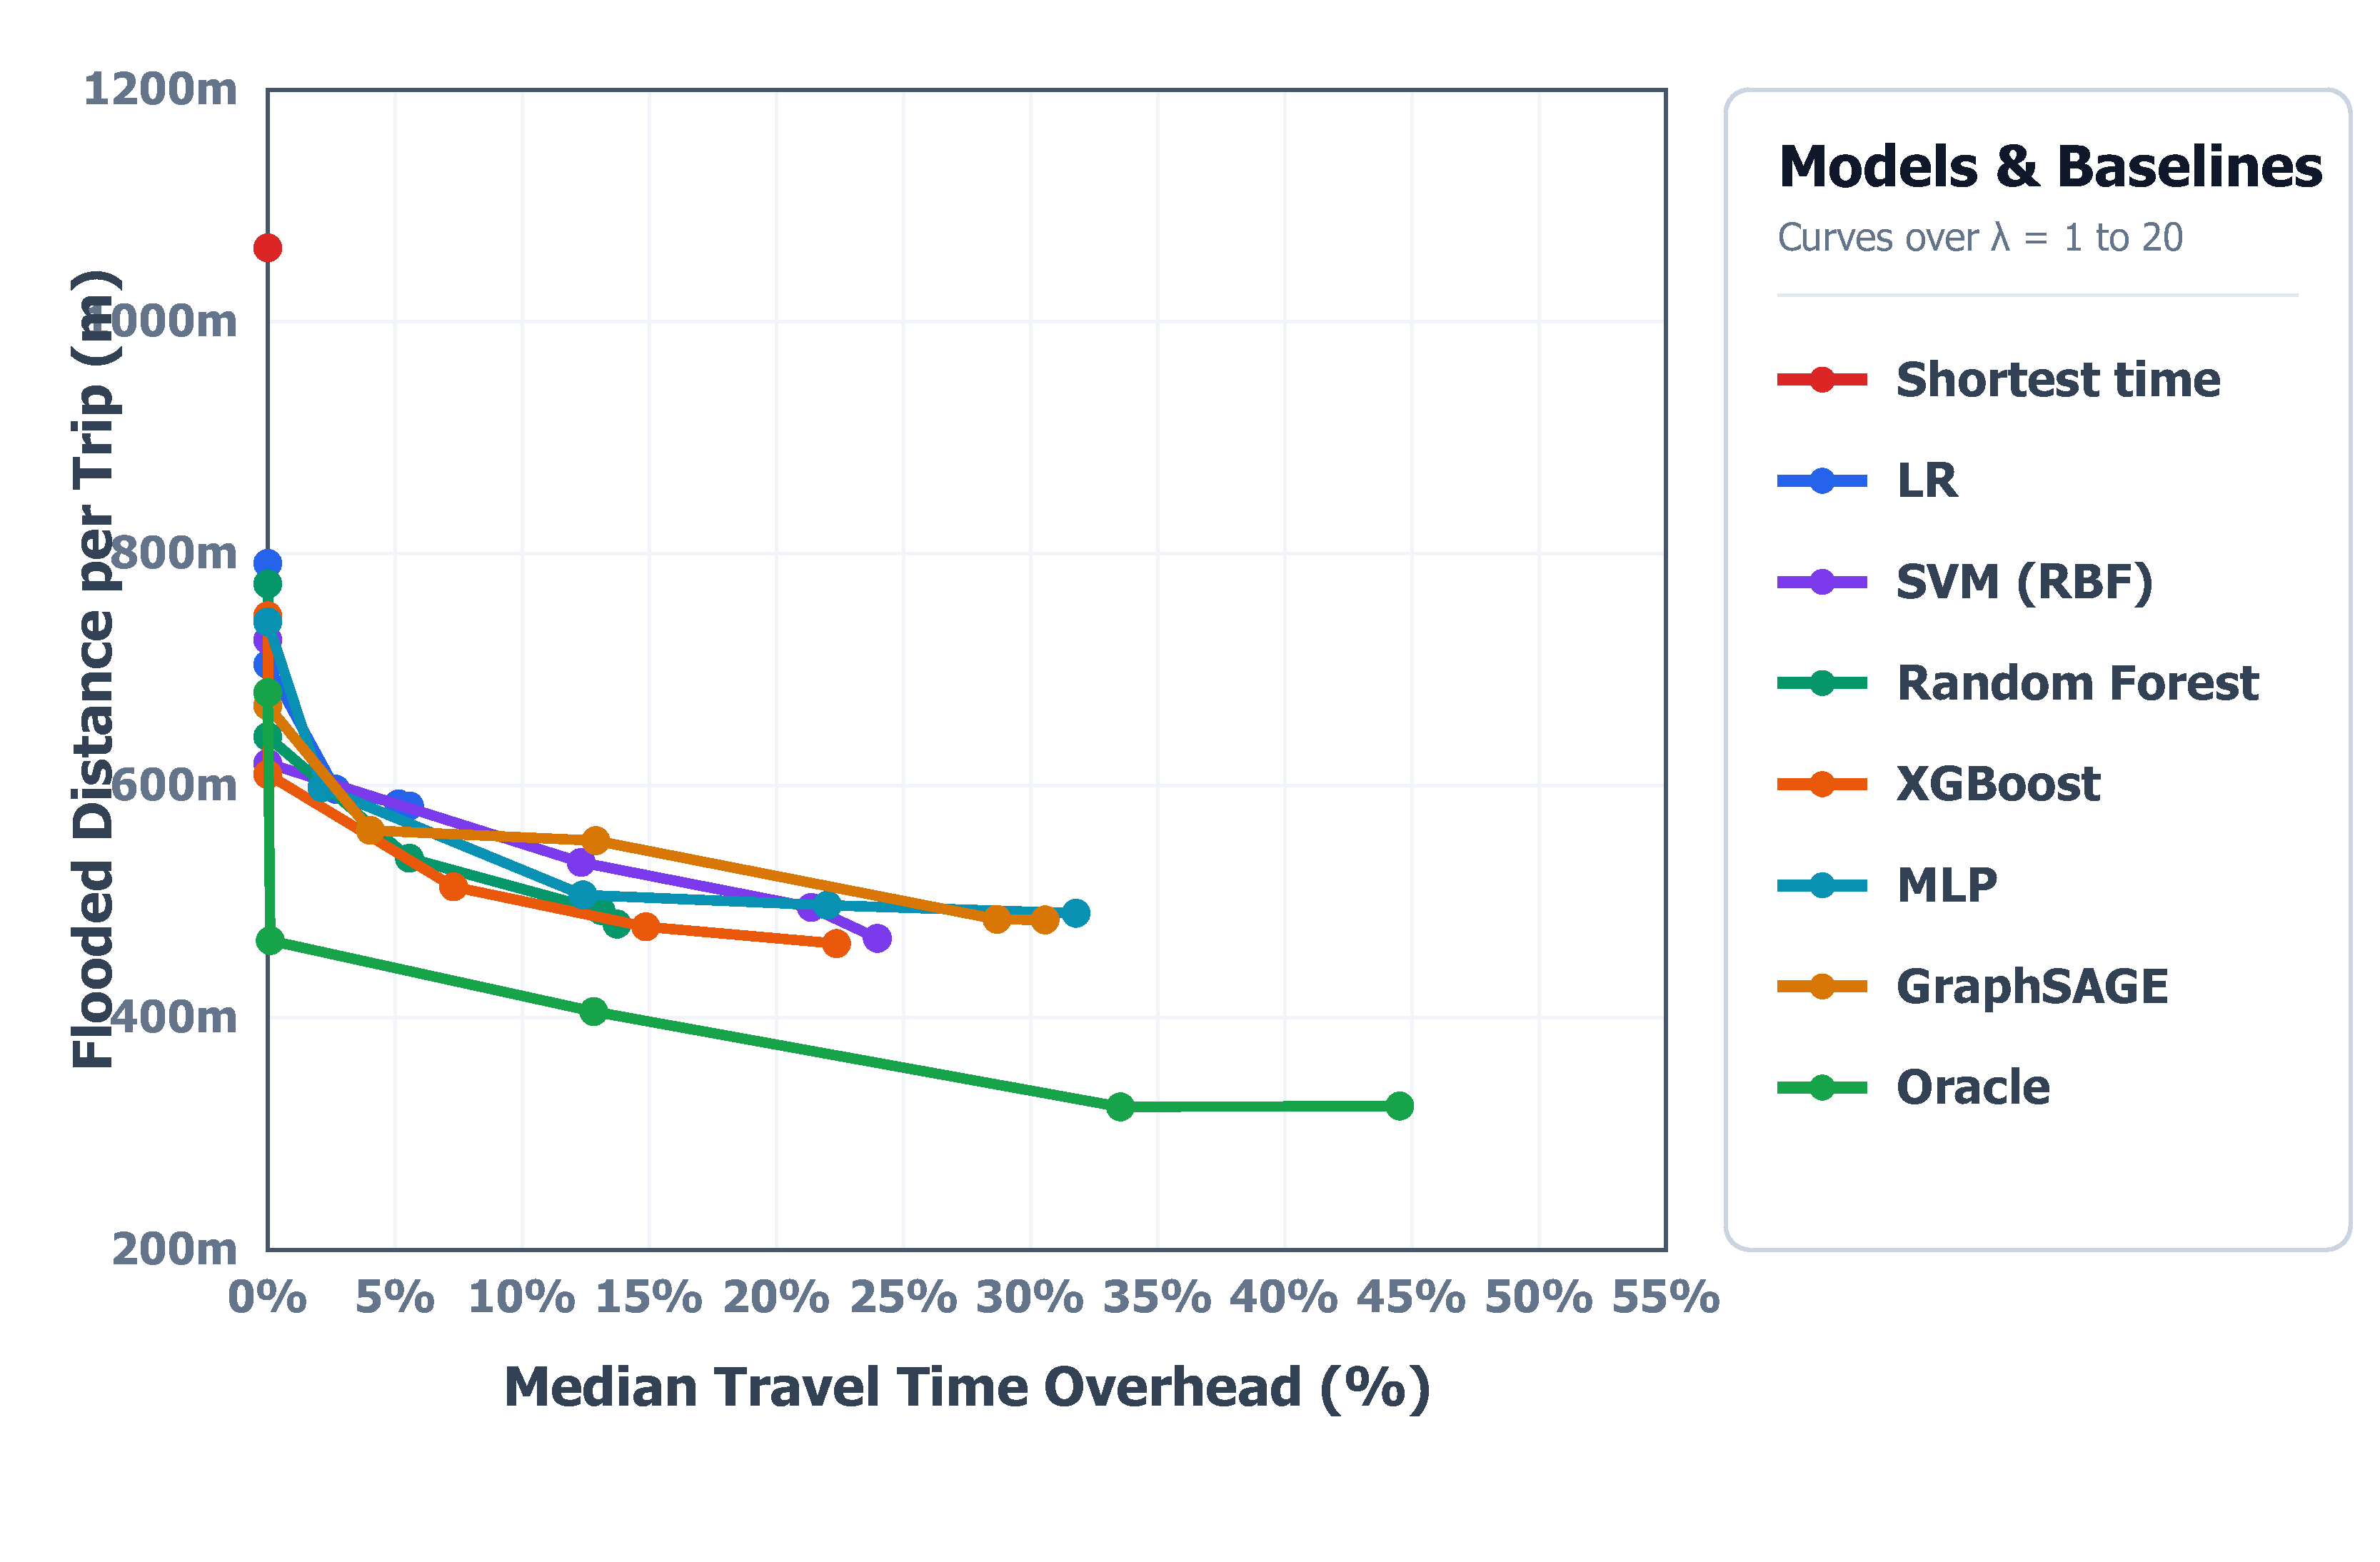
\includegraphics[width=\columnwidth]{fig8_lambda_tradeoff_curves}
  \caption{Trade-off between flood exposure and travel-time increase as risk aversion $\lambda$ varies from 1 to 20.}
  \label{fig:pareto}
\end{figure}

\subsection{Representative Route}
Fig.~\ref{fig:route} shows the routes of one representative OD pair crossing the central corridor, and Table~\ref{tab:route} lists their metrics. While the shortest-time path traverses 14 inundated segments (951.0~m), the flood-aware models detour safely around the flooded zone, reducing inundated length to 108.4~m (88.6\% reduction) with only 1.85~minutes of added travel time.

\begin{figure}[t]
  \centering
  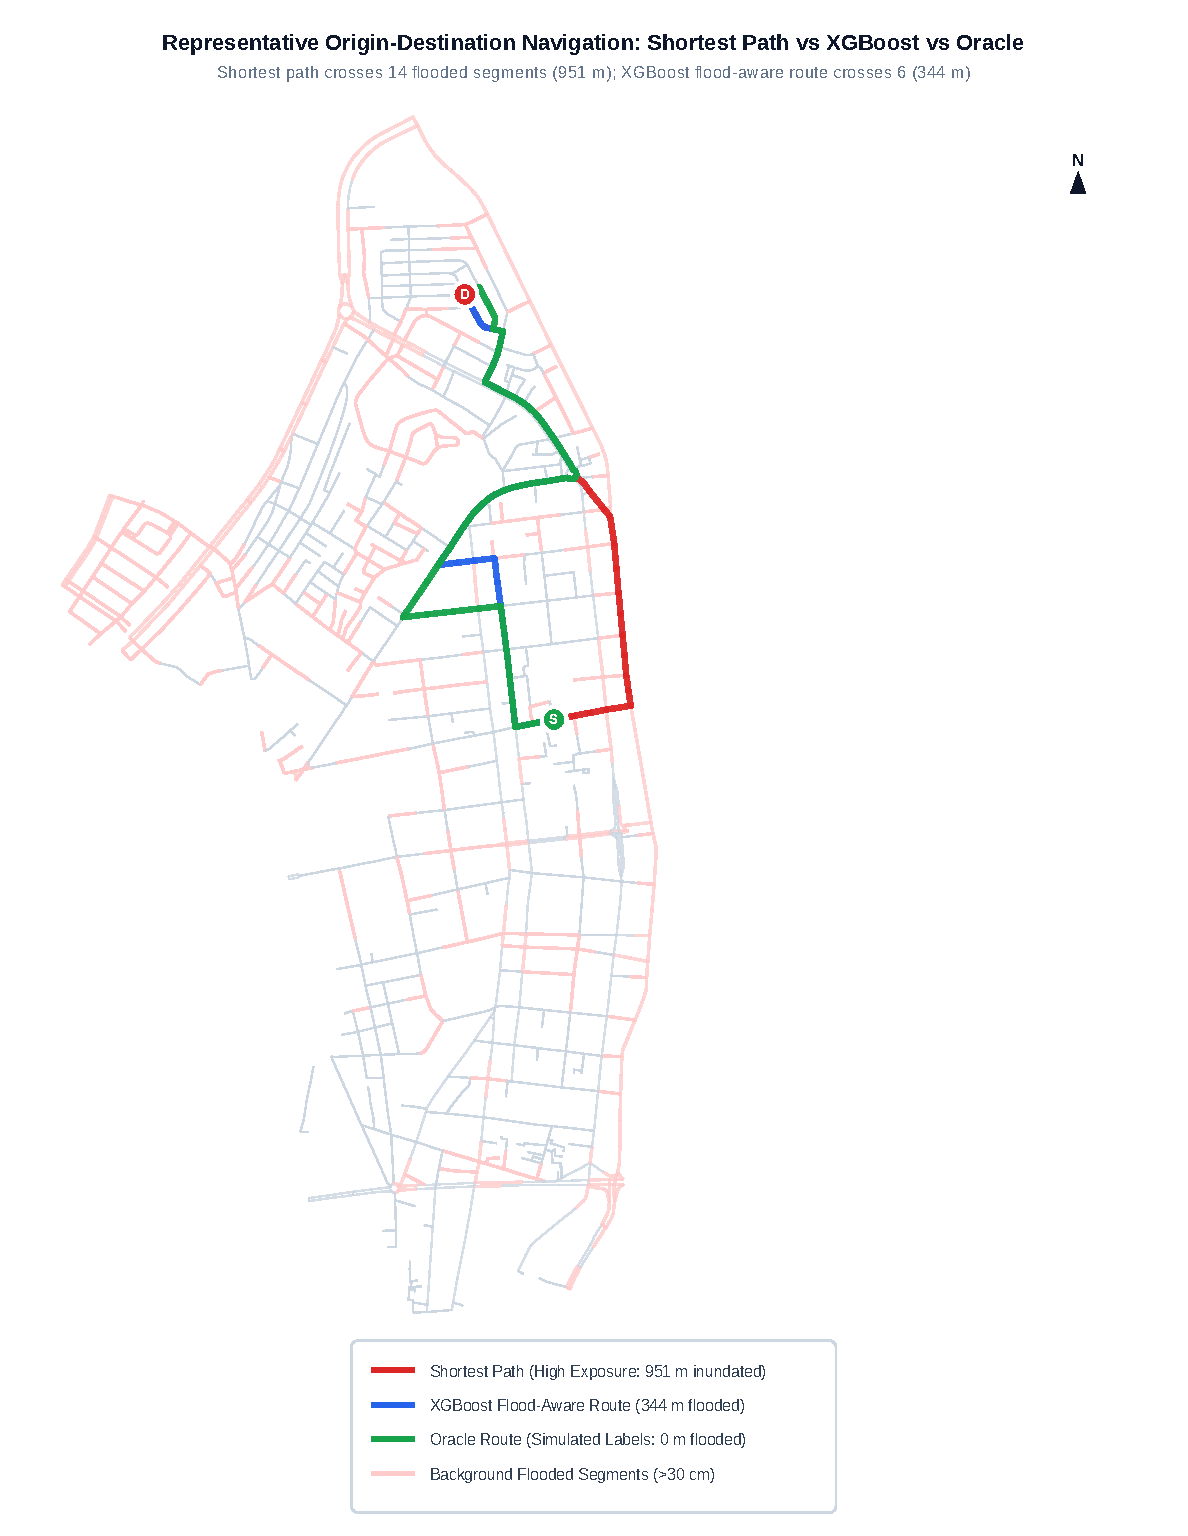
\includegraphics[width=\columnwidth]{fig9_representative_route}
  \caption{Routes for a representative OD pair: shortest time (red), flood-aware ML detour (blue), and oracle (green).}
  \label{fig:route}
\end{figure}

\begin{table}[t]
  \caption{Metrics of the Representative Route}
  \label{tab:route}
  \centering
  \footnotesize
  \setlength{\tabcolsep}{4pt}
  \begin{tabular}{lccc}
    \toprule
    Strategy & \shortstack{Travel\\time (min)} & \shortstack{Flooded\\segments} & \shortstack{Flooded\\length (m)} \\
    \midrule
    Shortest time     & 3.08 & 14 & 951.0 \\
    XGBoost           & 4.93 & 2  & 108.4 \\
    MLP               & 4.93 & 2  & 108.4 \\
    Oracle (observed) & 5.08 & 0  & 0.0 \\
    \bottomrule
  \end{tabular}
\end{table}

\subsection{Computational Efficiency}
Table~\ref{tab:efficiency} reports the size and run time of each model. Logistic regression is the fastest (0.01~s training, 12.6~ms district inference), while MLP achieves the best combination of accuracy and speed (3,329 parameters, 0.34~s training, 1.6~ms inference). GraphSAGE requires 0.52~s to train and 8.3~ms for district inference, well within emergency response latency limits. Routing execution averaged 4.2~ms per OD pair across all models.

\begin{table}[t]
  \caption{Model Size and Run Time}
  \label{tab:efficiency}
  \centering
  \footnotesize
  \setlength{\tabcolsep}{4pt}
  \begin{tabular}{lcccc}
    \toprule
    Model & \shortstack{Parameters} & \shortstack{Training\\time (s)} & \shortstack{Inference,\\district (ms)} & AUC-PR \\
    \midrule
    LR        & 19     & 0.01 & 12.6 & 0.840 \\
    SVM (RBF) & 37,062 & 0.34 & 97.4 & 0.856 \\
    RF        & 50,000 & 0.27 & 45.5 & 0.874 \\
    XGBoost   & 3,200  & 0.10 & 7.0  & 0.847 \\
    MLP       & 3,329  & 0.34 & 1.6  & \textbf{0.891} \\
    GraphSAGE & 3,297  & 0.52 & 8.3  & 0.867 \\
    \bottomrule
    \multicolumn{5}{l}{\scriptsize Routing time per OD pair: 4.2 ms for all models.}
  \end{tabular}
\end{table}

\subsection{Sensitivity Analysis}
\label{sec:sensitivity}
Fig.~\ref{fig:sensitivity} and Table~\ref{tab:sensitivity} show how the results change with spatial block size and the handling of uncertain segments. Model rankings remained stable across block scales from 250~m (AUC-PR 0.883) to 1000~m (AUC-PR 0.853). Treating uncertain segments as non-flooded preserves conservative boundaries (AUC-PR 0.847), while excluding uncertain segments yields 0.987 AUC-PR due to sharper class margins.

\begin{figure}[t]
  \centering
  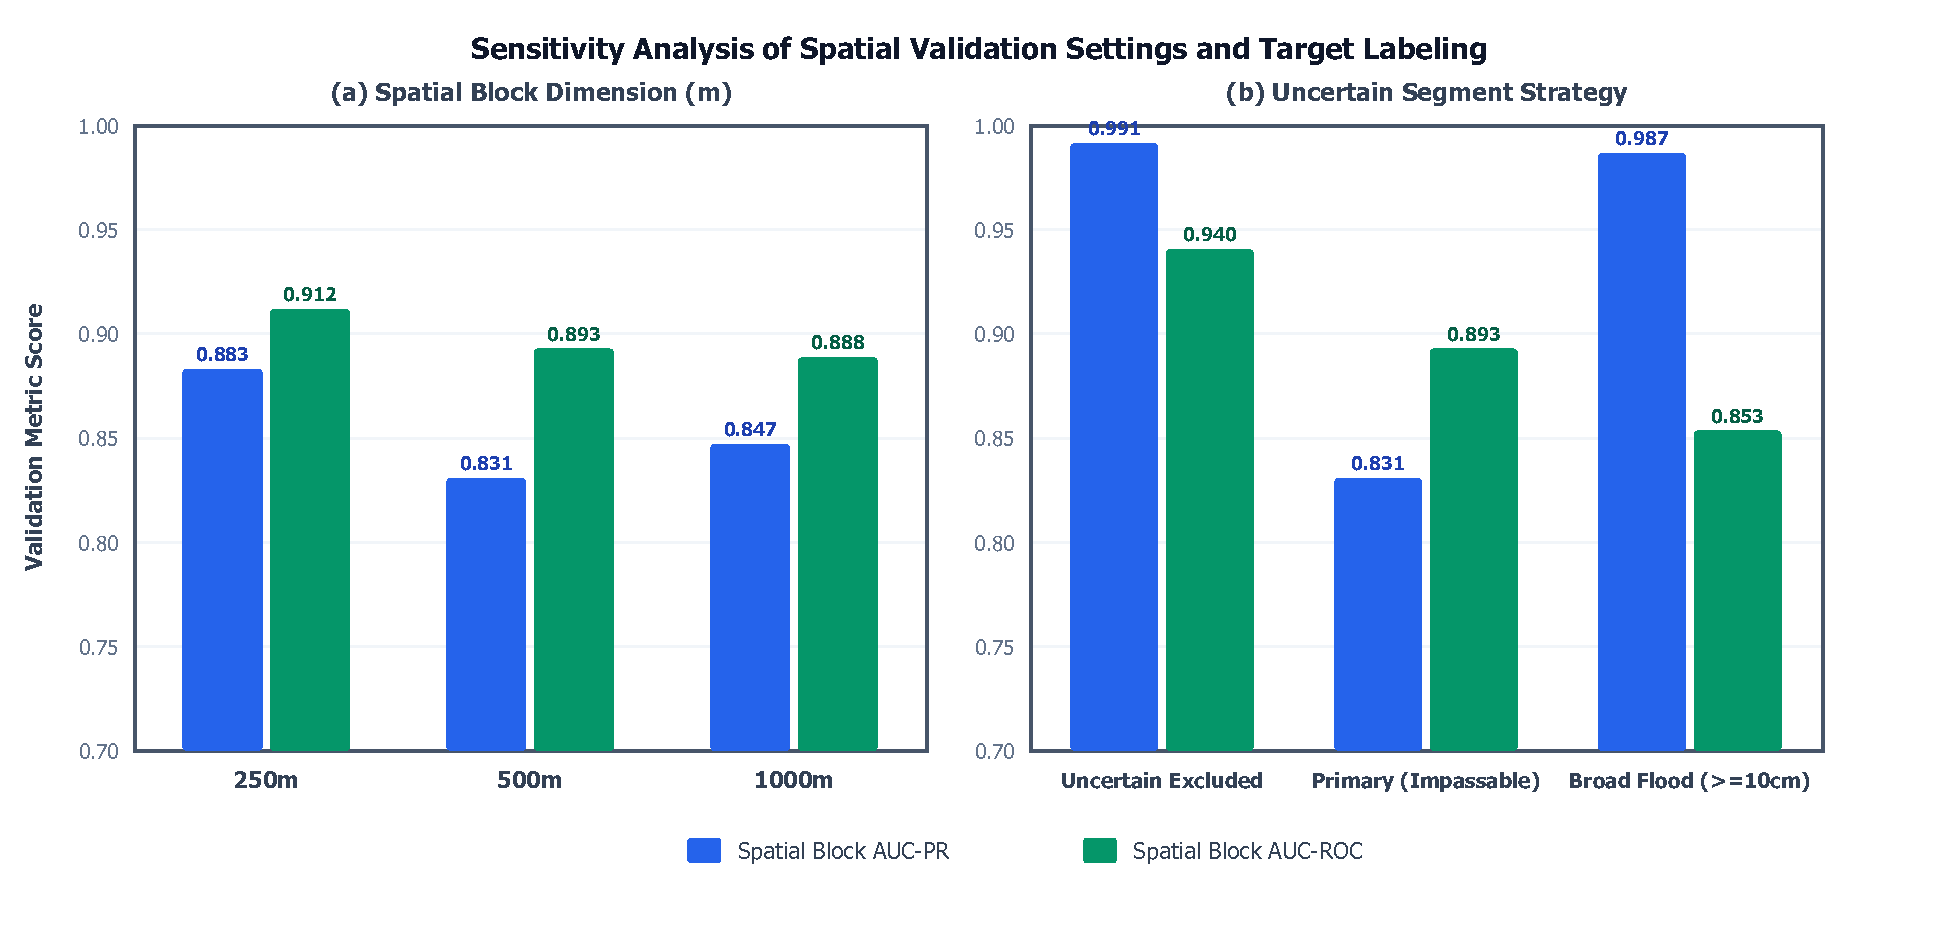
\includegraphics[width=\columnwidth]{fig10_sensitivity_analysis}
  \caption{Sensitivity of the results to (a) spatial block size and (b) handling of uncertain segments.}
  \label{fig:sensitivity}
\end{figure}

\begin{table}[t]
  \caption{Sensitivity of the Best Model to Validation and Labeling Settings}
  \label{tab:sensitivity}
  \centering
  \footnotesize
  \setlength{\tabcolsep}{4pt}
  \begin{tabular}{lccc}
    \toprule
    Setting & AUC-PR & Recall & Brier $\downarrow$ \\
    \midrule
    Block size 250~m                   & 0.883 & 0.839 & 0.131 \\
    Block size 500~m (main)            & 0.847 & 0.839 & 0.131 \\
    Block size 1000~m                  & 0.853 & 0.839 & 0.131 \\
    \midrule
    Uncertain segments excluded        & 0.987 & 0.955 & 0.053 \\
    Uncertain segments as non-flooded (main) & 0.847 & 0.839 & 0.131 \\
    Broad flood ($\ge$10~cm)           & 0.986 & 0.903 & 0.087 \\
    \bottomrule
  \end{tabular}
\end{table}

% !TeX root = ../main.tex
\section{Discussion}
\label{sec:discussion}

\subsection{Classification Scores and Routing Decisions}
The benchmarking results demonstrate that the top classification model (MLP, AUC-PR 0.891, recall 0.847) also achieved the superior routing outcome, reducing flooded segment exposure by 43.0\% and total inundated distance by 43.7\% relative to the shortest-time path. Conversely, models with lower spatial recall (such as Logistic Regression and SVM) or higher probability miscalibration (such as uncalibrated tree ensembles) incurred noticeably more flooded traversals. Because Dijkstra's routing decisions aggregate path-level risk penalties, even a few missed flooded segments (false negatives) can misdirect routes through inundated corridors. For practitioners, the benchmark indicates that models for flood-aware routing should be selected by their routing outcomes, or at least by recall and calibration, not by AUC alone.

\subsection{Flood Mechanisms}
SHAP importance rankings corroborate key physical flood mechanisms identified by hydrodynamic modeling in Da Nang~\cite{doan2023}. Depression depth and topographic position index emerged as the dominant features, followed by proximity to the Han River. During the October 2022 event, extreme rainfall coincided with high tidal river stages, inducing backwater ponding and disabling gravity drainage outfalls along the riverfront. The models accurately identified low-lying arterial underpasses (e.g., Dien Bien Phu) and riverbank road segments as high-risk clusters.

\subsection{Cost of Model Complexity}
Comparing model complexity against operational performance (Tables~\ref{tab:ablation} and~\ref{tab:efficiency}), MLP achieved the best balance of predictive accuracy and computation, requiring only 3,329 parameters and 1.6~ms for full district inference. GraphSAGE demonstrated the predictive value of topological message passing (+0.021 AUC-PR over the edge-free baseline) with an inference time of 8.3~ms. Given that all models evaluated completed district-wide inference well within 100~ms, the computational cost of neural and graph architectures is negligible compared to their gains in flood avoidance during routing.

\subsection{Limitations}
Five limitations apply. First, the study uses one event, so it identifies flood-prone segments rather than forecasting floods for any storm. Second, unreported flooding outside the excluded buffer is still labeled as non-flooded, which lowers the measured recall. Third, rainfall varies little across a single district, so it cannot separate segments within one event. Fourth, a coarse DEM may miss street-scale depressions. Fifth, crowd-sourced flood observations may introduce reporting bias toward major arterial corridors over smaller residential alleyways.


% !TeX root = ../main.tex
\section{Conclusion}
\label{sec:conclusion}

This paper benchmarked six machine learning models from five families for road-level flood prediction and flood-aware routing during the 2022 Da Nang flood. Multilayer perceptron (MLP) reached the highest AUC-PR of 0.891 $\pm$ 0.042 under spatial cross-validation, and as a routing cost it reduced flood exposure by 43.7\% for a 20.3\% increase in travel time. All models executed district-wide inference in under 98~ms, and their spatial rankings proved robust across block scales from 250~m to 1000~m.


Future work will add further events, timestamped depth records for short-term prediction, and risk costs in reinforcement-learning routing~\cite{le2026}. The risk maps could also provide prior flood probabilities for placing road sensors or cameras in Da Nang, following~\cite{pan2026}.


% ---------- Camera-ready only: keep hidden during double-blind review ----------
% \section*{Acknowledgment}
% \TODO{funding source and acknowledgements.}
% During the preparation of this manuscript, the author(s) used \TODO{tool} to improve
% grammar and readability. All content was reviewed and edited by the author(s), who take
% full responsibility for the published work.

\bibliographystyle{IEEEtran}
\bibliography{references}

\end{document}
